%%%%%%%%%%%%%%%%%%%%%%%%%%%%%%%%%%%%%%%%%%%%%%%%%%%%%%%%%%%%%%%%%%%%
%% I, the copyright holder of this work, release this work into the
%% public domain. This applies worldwide. In some countries this may
%% not be legally possible; if so: I grant anyone the right to use
%% this work for any purpose, without any conditions, unless such
%% conditions are required by law.
%%%%%%%%%%%%%%%%%%%%%%%%%%%%%%%%%%%%%%%%%%%%%%%%%%%%%%%%%%%%%%%%%%%%

\documentclass[
  digital, %% This option enables the default options for the
           %% digital version of a document. Replace with `printed`
           %% to enable the default options for the printed version
           %% of a document.
  table,   %% Causes the coloring of tables. Replace with `notable`
           %% to restore plain tables.
  nolof,     %% Prints the List of Figures. Replace with `nolof` to
           %% hide the List of Figures.
  nolot,     %% Prints the List of Tables. Replace with `nolot` to
           %% hide the List of Tables.
  %% More options are listed in the user guide at
  %% <http://mirrors.ctan.org/macros/latex/contrib/fithesis/guide/mu/fi.pdf>.
]{fithesis3}
%% The following section sets up the locales used in the thesis.
\usepackage[resetfonts]{cmap} %% We need to load the T2A font encoding
\usepackage[T1,T2A]{fontenc}  %% to use the Cyrillic fonts with Russian texts.
\usepackage[
  main=english, %% By using `czech` or `slovak` as the main locale
                %% instead of `english`, you can typeset the thesis
                %% in either Czech or Slovak, respectively.
  german, russian, czech, slovak %% The additional keys allow
]{babel}        %% foreign texts to be typeset as follows:
%%
%%   \begin{otherlanguage}{german}  ... \end{otherlanguage}
%%   \begin{otherlanguage}{russian} ... \end{otherlanguage}
%%   \begin{otherlanguage}{czech}   ... \end{otherlanguage}
%%   \begin{otherlanguage}{slovak}  ... \end{otherlanguage}
%%
%% For non-Latin scripts, it may be necessary to load additional
%% fonts:
\usepackage{paratype}
\def\textrussian#1{{\usefont{T2A}{PTSerif-TLF}{m}{rm}#1}}
%%
%% The following section sets up the metadata of the thesis.
\thesissetup{
    date          = 2017/01/04,
    university    = mu,
    faculty       = fi,
    type          = mgr,
    author        = Bc. David Kouřil,
    gender        = m,
    advisor       = Ivan Viola and Barbora Kozlikova,
    title         = {Maya2CellVIEW: Integrated Tool for Creating Large and Complex Molecular Scenes},
    TeXtitle      = {Maya2CellVIEW: Integrated Tool for Creating Large and Complex Molecular Scenes},
    keywords      = {molecular visualization, illustration, Maya, Unity, ...},
    TeXkeywords   = {keyword1, keyword2, \ldots},
    bib           = example.bib,
}
\thesislong{abstract}{
    Scientific illustrators communicate the cutting edge of research through their illustrations. There are numerous software tools that assist them with this job. The aim of this thesis is to push abilities of illustrators working on a large scale molecular scenes. This is done by connecting two software packages - Maya and cellVIEW - combining the rendering possibilities of cellVIEW and modeling tools of Maya which results in more effective and efficient workflow. 
}
\thesislong{thanks}{
    This is the acknowledgement for my thesis, which can

    span multiple paragraphs.
}
%% The following section sets up the bibliography.
\usepackage{csquotes}
\usepackage[              %% When typesetting the bibliography, the
 backend=biber,          %% `numeric` style will be used for the
%  backend=bibtex,
  style=numeric,          %% entries and the `numeric-comp` style
  citestyle=numeric-comp, %% for the references to the entries. The
  sorting=none,           %% entries will be sorted in cite order.
  sortlocale=auto         %% For more unformation about the available
]{biblatex}               %% `style`s and `citestyles`, see:
%% <http://mirrors.ctan.org/macros/latex/contrib/biblatex/doc/biblatex.pdf>.
\addbibresource{example.bib} %% The bibliograpic database within
                          %% the file `example.bib` will be used.
\usepackage{makeidx}      %% The `makeidx` package contains
\makeindex                %% helper commands for index typesetting.
%% These additional packages are used within the document:
\usepackage{paralist}
\usepackage{amsmath}
\usepackage{amsthm}
\usepackage{amsfonts}
\usepackage{url}
\usepackage{menukeys}
\begin{document}
\chapter{Introduction}
%[\textbf{In what field are we? What are the people in this domain doing?}]
In this day and age, scientists come to new findings everyday. Unfortunately, not all of these are ever shown to the general public. This can be because of several reasons. New facts might not be easily visualizeable. Or the things that they found out are a piece of a bigger picture and hence cannot be easily communicated. On top of that, scientists are not usually trained to expose their results to the public eye.

This is the job of scientific illustrator. These people are, first and foremost, experts in their fields but on top of that they have invested significant amount of time on acquiring and perfecting their artistic skills. They use these skills to visualize the science in their domain with easily understandable images, animations or other forms of media. To name just a few examples - Drew Berry \cite{DrewBerryMovies}, Graham Johnson \cite{GrahamCellVideo}, Janet Iwasa \cite{iwasa2010animating}.

% TODO: [\textbf{why are illustrations/animations useful: what art was talking about and also janet in molecular flipbook video}]

There are many ways how they can do their job. Few years back, illustrations have been done by hand - with traditional drawing and painting methods. This is a very timely process, as individual illustration can take months to make. An example of an artist who still uses these traditional techniques we can name David Goodsell []. Goodsell has developed a style of abstracting details while preserving the general shapes. However, this is a very timely process, as individual illustration can take months to make \cite{DavidGoodsellVideo}. If we consider that science is moving way faster what could end up happening is that before an illustration is finished a new finding emerges, rendering the illustration effectively obsolete. This is of course undesirable and scientific illustrators have been looking for ways how to accelerate this process.

%[\textbf{Can we use computer graphics for this?}]
Then came the age of computer graphics. As graphics tools have become more and more common and sophisticated in a field of computer generated movies (reference to Pixar?). Tools have become more accessible, easier to use and so scientific illustrators adapted and tried to use these tools for their benefit. Tools like Maya, Cinema4D, or XXX are nowadays the industry standards when it comes to authoring 3D content. Inside these programs there usually exist a software called renderer. With this two parts - modeler and renderer - the user is able to create images or animations (movies) from the 3d data that he creates in the software.
Even with just this, the modern computer graphics brings us the possibility to create amazing imagery and enables illustrators to show ordinary people fenomena from all kinds of science disciplines.

%[\textbf{Are there any problems that we could solve?}]
But this workflow isn't very effective. One of the obstacles in the work of illustrators is that the software they are using is made for somebody else. Games and movies industry are the leading industries that push computer graphics tool creators forwards and provides most of the revenue for them. This means that these tools, no matter how much they try to be versatile, are being skewed towards the use cases of movies and games industries. That means that people who want to create scientific content might struggle to use the tools sometimes.

For this, there are other tools that help them to make the pipeline more effective. This doesn't mean that these tools completely replace Maya or Cinema4D. The domain specific tools are more commonly implemented in a form of a plugin that is developed and loaded into the concrete software packages.

In the end - the features that 3D authoring package provides for modeling 3D scenes are hugely beneficial to the creators. Another things is - people that used these software are used to that and switching from one to another is not a matter of a short time. That's one of the things that we need to take into account. The pipeline of each artist might be a little different and rather than suggesting a solution that completely replaces their pipeline, it's better to make a tools that doesn't break their workflow but rather the artist is able to incorporate the tool, benefit from it but doesn't have to change the way they work a lot.

% [\textbf{what are the alternatives to what people are using already?}]
There also exist programs that are completely separated from any of the mentioned authoring software. There is an active research in the domain of visualization, with many conferences every year and thousands (?) of research papers in this domain. Usually, as a biproduct, these paper generate software that showcases the proposed visualization technique or pipeline. Some of these developed into full featured visualization packages and thus provide a way how to illustrate something in a new way. While these programs might hugely benefit scientific illustrators, it's not always the case that they get used. This might be because of several reasons one of which is that the illustrators are simply used to a certain pipeline and incorporating a new software into this pipeline doesn't seems very beneficial to them. Another problem is that because these programs are developed for a certain use cases (showcasing the point of the paper) they might not be easily appliable to more than one purpose.

[\textbf{``mission statement'' of the thesis}]
In this thesis, we made an effort to solve these problems. Our domain of choice is molecular visualization.

In this domain we try to visualize living (?) organisms on the smallest possible scale. With this approach, the computer memory and performance requirements are very challenging even for todays available hardware. Still, people have been able to visualize for example model of HIV in blood plasma in it's full detail down do individual atoms of each protein. This however, is achieved by using a very customized rendering method and a custom data format. In 3D graphics, data are usually represented as meshes consisting of triangles (which in turn are made of vertices). If we wanted to represent each atom as a sphere, we would need at least <number> of vertices for one atom and that's only for the roughest level-of-detail. With such representation, a one whole protein could use up to X bytes of memory which already takes up most of the video cards' memory. Thus this representation is not suitable for this task. Instead, various other techniques have been developed for rendering on molecular data.

That being said, these techniques are not usually taken into account when 3D authoring software is developed. As was mentioned, the primary users of these software are video games and movies industry, where mesh representation is the one used. That implies that people that use these programs don't have access to the cutting edge technology of rendering, visualization and illustration of molecular data and there is room for us to improve this situation.

In the next chapter, we will describe the state of the art tools that are used for molecular visualization today and we'll mainly focus on showing the gaps in intercompability of the available programs. Then, in chapter 3, we will propose a method of how the problem could be solved.

\chapter{State of the Art}
%I think the sections could be: 3D Modeling Software (Maya, C4D), Niche (Specific) Tools (cellVIEW, ...), Data Generation (cellPack)
%Popsat: Molecular Flipbook, Molecular workbench, molecular maya, mcell, cellblender, pymol, VMD, ePMV(scripps)

In this chapter we will introduce the software that is currently available for scientific illustrators working in molecular visualization. Illustrators have gone a long way from doing these works by hand and nowadays there exist a variety of programs that help them do their job communicating the scientific findings. However, as we will see there is are multiple level of user accessibility and different programs have different prerequisities on the level of expertise of its users. Given the fact that when communicating science one has to understand to a certain extent the science there are multiple ways to approach the design of the program. We also see that the

\section{Commercial 3D Software}
%[\textbf{Commercial 3D software is absolutely dominating}]
First and foremost, the pipeline of almost all of these illustrators is strongly built upon a 3D modeling software of their choice. The biggest players right now are Autodesk Maya, Cinema 4D, Autodesk 3Ds Max Design, although other solutions have started to emerge - we can name open-sourced Blender or more and more popular MODO(https://www.thefoundry.co.uk/case-studies/viscira/). Maya and Cinema4D are the dominating choices between illustrators. These programs are complex and aim to provide tool for all kinds of users. Their main functionality revolves around two activities - creation of the 3D scene which is most commonly a mesh model and rendering of this scene. These two stages will be referred to as modeling and rendering.

%[\textbf{things that are nice to have from these programs - easy manipulation with objects, scene graph to organize the scene, tools for animation, semi-automatic object positioning (random, particles)}]
Disregarding the differences between all the 3D software of this kind, there are some key features that are more or less contained in all of them. First, objects in scenes are organised into some variation of ``scene hierarchy'' or ``scene tree''. This allows users to organise their objects and establish parent-child relationships between these objects. Second, navigation in the 3D scene is always solved. Every named program allows the user to open multiple viewports at the same time where every viewport shows different camera position. Third, object manipulation - translation, rotation and scale - is solved and made available under shortcut which allows the illustrator/animator to work efficiently.
These are the killer features and even though they are present in all of the programs, the illustrators are often used to the way they work or to a certain shortcut which means that it's not trivial for them to switch from one to another (or it is but it takes some time).

%[\textbf{scientists have to go through training to be able to use these programs}]
All of these programs are big and complex. This comes from the fact that they are meant to be general tools for anybody who needs to manipulate 3D models and create images or movies out of it. Therefore, mastering this tool, or even getting on proficiency level enough to produce meaningful work, is not an easy task and takes between several months to years. This amount of time is something not a lot of scientists are willing, or even able, to sacrifice. However, as we said in the introduction, by having the information compiled into visual form is hugely beneficial so some people were willing to dive into learning these tools and have been able to use them to an incredible benefit. Ideally we would like more scientists to be able to create visuals like this so attempts to simplify this process have been made.

\subsection{Plugins}
%[\textbf{We have an ``entry point'' which we can exploit to inject our custom functionality}]
Luckily, it has become a convention that all of these 3D programs provide some kind of scripting interface. This enables its users to extend the program with plugins that use the scripting interface. This way the user can implement functionality that he or she is missing from the basic program. Thanks to that these 3D authoring programs can be adapted to more use cases.

[\textbf{Tools where people already used this plugin architecture}]
Some of these plugins have actually already been implemented to help artists in molecular illustration. The most prominent is Molecular Maya which, as the name suggests, extends Maya with the ability load and manipulate models of macromolecules from Protein Database. Molecular Maya plugins gives its users the ability to load macromolecules based on its PDB ID or locally from pdb file. After the model is loaded, user is able to select the display representation (between TODO: vyjmenovat) and also select with how much detail the model should be rendered.

Similar plugin exists for Blender modeling program as well. It's name is cellblender
This could be a nice reference: https://pdb101.rcsb.org/learn/resource/molecular-animation-q-and-a-interview
[\textbf{How people normally render - offline}]
The rendering stage takes place after the scene is modelled. Again, there are more options at hand. 3D packages usually come with a default rendering solution which is for the most part good enough to use. For more demanding artist, external renderers like vray, mental ray, corona or octane. What these renderes have in common is that they are so called ``offline renderers''. In practice this means that they are using ray tracing (or similar) technique to render the scene with a process that is very much close to how light works in real life. The disadvantage of this approach is that this process take more time. It usually isn't possible to achieve real-time rendering (fps at least 25).

[\textbf{Define the workflow - how it is now and how we could improve it (fasten it)}]
We should mention here how the workflow of artists looks like. The individual stages - modeling and rendering - don't happen one after another. The workflow actually looks more like a loop with multiple interactions. The final rendered image is essential when creating the actual scene as the artist needs to tweak multiple attributes of the scene to make it look like he wants. In practice, this means that he performs this modeling/rendering iterations very frequently. Thus he needs this iteration loop to be as fast as possible. As the renderers are getting better and computer hardware more and more powerful, the iterations are getting shorter. (Octane-like) renderers are contributing to this as well. They work in a way that they first display some aproximation of ligthing of the scene (primary rays) and iteratively increase the quality of rendering. User can therefore see the effect of changes he's made in the scene sooner. However, when we talk about molecular visualization we don't usually care about the rendering quality and physical correctness. What we usually use are simpler, almost illustrative rendering styles. Thus we can simplify the techniques to the point of being able to render molecular scenes in interactive frametimes (real-time) which brings us the possibility to create interactive molecular scenes. This is hugely attractive for scientific illustrators.

[\textbf{interactive renderers like octane, how do they fit and why they are not the full solution}]
In recent years, interactive renderers have been gaining popularity. These tools work in a similar way as did previously offline renderers. The difference is that they show the artist an intermediate result of the path tracing (or the technique they are using). This way the artist gets a fast render of his scene with a lower quality and the quality of this image is refined iteratively. This approach also enable its user to see changes in the scene in a quick preview and as it is right now, a lot of artist have been using this feature and they say it's been greatly helping them in their work. There is however one thing that we can still improve. These renderers still operate on meshes. We've already talked about how our data can be efficiently simplified to our purpose and therefore rendered with a great performance in real-time. Thus even if interactive renderers like Octane could improve the workflow we can still provide a better performance by using custom renderer like cellVIEW.

\section{Domain-specific tools}
%kinemage (http://kinemage.biochem.duke.edu/), chimera (http://www.cgl.ucsf.edu/chimera/), jmol?
[\textbf{intro}]
In the field of molecular visualization, numerous programs exist. They share a lot of features but they each have their own specialities and are meant to be used for slightly different tasks. We will name a few that have been developed for some time and have matured to a certain extent. Other than that, other tools exist which are even more specialized. These might be results of a research and they accompany a paper describing the technique. This means that these programs are not that well usable out-of-the-box but rather serve as a demonstration of a certain technique.

\textbf{Molecular Flipbook}
One of the more user-friendlier and easier to use tools is Molecular Flipbook. It has been develoved by a team lead by Janet Iwasa and it consists of two parts - an animation program and a website where creators can share their works. The main motivation for this project is to create tool that even scientists without education in animation can use to communicate their ideas through simple molecular animations. They achieve this by building the program around the concept of simplified key-frame animation technique. The website portion of the project is meant to serve as a database of animations explaining various processes. Creators can upload their works and improve works of others.
[\textbf{TODO:} cons, done on top of a blender game engine, info: http://mikepan.com/flipbook.html]

\textbf{Molecular Workbench}?

\textbf{PyMol} is a more mature project which aims to be used by more expert users. It is an open-source software product in which the user can view, render, animate and export 3D molecular structures. PyMOL can visualize molecules with several representations - spheres, surface, mesh, lines, sticks, etc. Rendering can be done with internal ray caster. Based on Python.

\textbf{VMD} (Visual Molecular Dynamics) serves as a tool for modeling, visualization and analysis. It actually has a long tradition, bening first introduced in 1996.

\textbf{cellVIEW} is a tool with the ability to render large biological macromolecular scene at an interactive frame-rate. It has been designed and implemented with regards to this use case with the use of state-of-the-art rendering techniques. It employs several modern techniques to reduce the amount of processed geometry in macromolecular scenes to provide its users with a real-time performance. As a result cellVIEW can render scenes containing up to several billion atoms with a framerate above 60 fps (?). cellVIEW has been implemented with Unity game engine. The rendering styles has been inspired by illustration by David Goodsell who has developed a style of abstracting the shape of individual proteins to reduce visual noise of the picture. cellVIEW immitates this approach by integrating a level-of-details scheme - the farther the protein is from the camera the less amount of its atoms are rendered and the rendered atoms are scaled up. This approach results in a multiscale visualization - user can zoom in to see individual atoms of a protein instance, or he can zoom out and see the whole dataset with its distinguisable compartments. The biggest dataset that has been possible to visualize is HIV, however tests have been done and it should be possible to render e-coli bacteria (which is X times larger)

\textbf{ePMV} is a very interesting project that is trying to solve a similar problem as we do. Uses uPy. We don't use Python. Our method is more general (?).

\section{Data Generation}
[\textbf{cellpack}]An important part of any scientific illustration are the data one is trying to illustrate. In the case of molecular models, there is cellPACK which helps us with this. cellPACK is a software that assembles large molecular scenes from a description (a recipe) of how this scene should look, what it should contain and in what quantity.

\section{File Formats}

[\textbf{are there any standardized file formats in this field?}]In computer science there are not a lot of ways to translate information from one program to another. The majority of this communication is done via files that are exported on one side and imported on another. This lead to a need for standardized format in which this data are formatted so that both of these programs understand each other. TODO: write about standard format in molecules (not a lot - pdb, we are taking advantage of that, other than that, maybe write about packing result data file format) This simple approach is fine for most of the application where it's used. In our case however this isn't sufficient. There is one big problem. If user needs to perform the actual export and import step, this greatly reduces his productivity. Another problem that is found in our domain has already been mentioned - rendering times.

\chapter{Method}
%[image: modeler, renderer, illustrate the connection through shared memory, data streaming, camera position]

%[\textbf{we focus on fastening the workflow by using our renderer}]
As was discussed in State of the Art chapter, the majority of artists uses commercial 3D software. These programs are very good at modeling and rendering 3D content as a set of meshes - 3D objects consisting of triangles. However, for molecular data and scenes, mesh is not the best representation and there exist rendering techniques that perform way better if we use other representation.

%[\textbf{we can take advantage} of the fact that illustrators use illustrative style, simplified and the data is very compact actually so we can provide them the interactive preview]
Another thing we can take advantage of is that illustrations and animation describing structures and function of objects at nano-scale don't often profit from using ultra-realistic rendering. They show concepts that are happening at different scales than the stuff that programs are usually made for. Thus they usually want to use more illustrative, simplified, rendering styles.

In our use case, this is even more true because we are dealing with a very dense data sets. We want to simplify what we show to reduce the visual noise in the ouput image. Various level-of-detail (LOD) schemes exist and they not only help with filtering of the visual noise but also reduce the performance requierements.

Thanks to these simplifications we can render molecular scenes with interactive framerates, as has been shown by cellVIEW[ref]. Unfortunately, these techniques are not implemented in 3D commercial programs which is what the artists usually use. Our goal is to make it so that the artist can use his software of choice to model his scenes but also take advantage of modern rendering. The use is two-fold: real-time rendering can serve as a preview of the scene but also can be used as a final result. The goal of this project was to come up with an idea of how to connect these two programs so that they will work together.

\begin{figure}
  \centering
  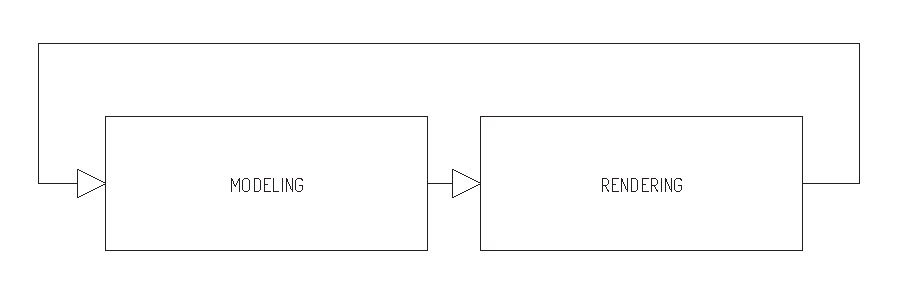
\includegraphics[scale=0.8]{images/pipeline.pdf}
  \caption{workflow}
  \label{fig:workflow}
\end{figure}

%[\textbf{two options, we choose third}]
Ultimately, we have two programs and we want to use some functionality from the first one and other functionality from the second one. The naive solution would be to implement our desired functionality into the software that is missing it. In our case, that would mean we could either implement the fast and visually appealing rendering into our modeling software, or we could do the opposite and implement the desired modeling tools into our renderer.

The problem with the first option is that most of the 3D software packages that artists are using the most are commercial solutions with closed source code. It is possible to extend them via API that they usually provide but that is not enough if we want to implement state-of-the-art technique that sometimes requires the most modern technology in terms of graphics API etc.

We've chosen to go with another, third, option. We don't want to reimplement from scratch something that is already available to use. We want to avoid this development overhead. Instead, we went for a different approach and tried to connect the two parts in a way that would allow us to use both features at the same time. We do this by using both of the programs and establishing a communication channel between them. We use writing and reading from shared memory to accomplish this communication. In our case the communication is one-way. We have a modeled scene on one side and we want to transfer data describing this scene to have it rendered on the other side. As we will show this can be done in a straight-forward fashion as our scenes can be simplified to the point when we can describe them with few numbers.

%[\textbf{why is it that we can do this?}]
We can establish such communication between the two programs mainly thanks to the character of the data we are dealing with.

%[\textbf{the data}]
Scenes we work with consist of macromolecules - proteins and lipids. Macromolecules in turn are made of atoms of different elements. There are multiple representations by which we usually visualize atomic data (see chapter State of the Art) [TODO: where should I put this?]. However the underlining data doesn't change. An instance of molecule is defined by the type information (what kind of molecule this is), position and rotation of the instance, and last, a list of atoms that this molecule is made of.

% we will use some placeholder geometry in maya
On the side of modeling program, we want to see an approximation of the scene. One way would be to use a simple geometry like cube or sphere as a placeholder for each molecule. Such placeholder would then serve as an object that we manipulate instead of an actual molecule. We tried something a little bit different. With Molecular Maya plugin, we can load a molecule description in form of a pdb file. With the same plugin it is also possible to generate a polygonial surface mesh representation with choosable detail level. We therefore load a molecule and generate very low resolution mesh which serves as our placeholder.
% TODO: IMG: show low poly model of a protein generated with mol maya

%[\textbf{overview of the method: two ends, shared memory, what needs to be transfered, ...}]
On the Figure X, you can see an overview of the system. On one side we have a modeling software while on the other we have a domain-specific tool, in our case it's a high performance renderer. Our vision was to have both of these programs running at the same time. The illustrator could have his scene opened in his modelling software. This way he would be using the tools he knows and is accustomed to for modelling the actual scene. Then on the renderer side he would be able to see how the changes he's made are reflected in the rendered final image. This all would happen in real-time thanks to writes and reads into and from shared memory.

% [\textbf{simplifications, how the scene can be described}]
As was already mentioned, when dealing with molecular data we can take advantage of several simplifications. A scene like this consists of macromolecules: proteins and lipids. First simplification - we consider the shape of the molecule to be static. This means that inside each molecule, the positions of all the atoms doesn't change in time. The position of the atoms is taken from the PDB file. The second simplification is that all the instances of certain molecule type look the same. They only differ in position and rotation.

% [\textbf{what data do we need to transfer}]
With these facts in mind, we can define a molecular scene as a set of molecules, where each molecule is defined by its position, rotation, and type, which says what kind of molecule this instance is.

This means that we need to stream this data - positions, rotations and types - of all molecule instances from the modeling software to the rendering tool. Because of the technical implications we write the data in a format described on Figure X. This is more efficient that writing the data in a format position/rotation/into for each molecule.
\section{Process}
\subsection{Parsing the Scene}
% [\textbf{the actual process}]
Inside the modeling software, we scan the scene, looking for molecular objects. We need to identify an object which is supposed to represent an instance of a molecule. We find out what type of molecule this is. This information is saved in a form of pdb id. For each of the found instances we also read its world position and rotation. This info is accumulated into an array and then prepared to be written into the memory.

There are several approaches and optimizations possible at this level and these depent mostly on the API that the modeling software provides. We were able to inject this method into a callback which is called everytime a scene has changed. After this happens, we scan all the models in the scene and look for molecular objects. This could be optimized in a way that only the objects that have changed report their changes. That way not all the object in the scene need to be scanned which saves us some performance. As we've discovered however, the APIs are not always keen on having such a performance-heavy procedures executed on each frame and so the concrete implementation heavily depends on the chosen modeling software and its API. We will describe in more detail how we accomplished this with Maya API in the chapter Implementation.

\subsection{Writing into and Reading from Shared Memory}
Once the data about current state of the scene is accumulated into position, rotation and info arrays, we can write these into the shared memory. Operating system api calls should be used for this. Again, for more details, see chapter Implementation to see how we did this on Windows operating system.

\subsection{Using the data}
Reading the data uses operating system api calls as well. In our case, because we are operating on the interface between c++ and c\#, the code that reads from the memory is pretty simple, only retrieving memory address and sending it into the c\# part of the system. This data is then copied into buffers inside cellVIEW which in turn sends them to GPU for render. We format the data in a way so that there is no additional manipulation on the data between these steps required. After the data write, we ideally want to only copy the chunks of memory from one place to another.

%[\textbf{Why Maya?}]
We have chosen Maya as the modeling software because our collaborating partner, Drew Berry, is its prominent user and he's been a key person that we had in mind when implementing this method. Chosing cellVIEW as the renderer has been an obvious choice as its rendering capabilities are on the state-of-the-art level of what common hardware computers are able to render. Drew Berry has been impressed with the results of cellVIEW and expressed his interest in using it for his movies.

\section{old}

[\textbf{we don't want to use files} TODO: why?]Our method tries to solve these two problems. The problem of import/export is solved by using shared memory instead of files managed by the user. The rendering times problem is solved by using modern rendering techniques which enable us to render what we want in an interactive framerate.
The reason why it's possible to take this approach of using shared memory comes from the character of data that we work with. Molecular scenes consist of molecules. Molecules are made of atoms which can be, and usually are, represented as spheres. Atoms of different elements are visualized by having different radii and colors. So for every molecule we need to keep track of what atoms it consists of, positions of those atoms and type of each of those atoms. This is even more leveraged by Protein Data Bank, which stores data about various proteins that have been found through out the years. For us, this means that we only need to keep track of the type of molecule and by fetching data from Protein Data Bank we get information about the protein cataloged under the protein identifier. Our scenes are (simplified) made of macromolecules. That means that in the end for rendering the scene we need a list of molecules, where for each molecule instance we need to save it's position, rotation and type. That's all the info that we need to be able to render our large molecular scenes. Even though this is still a lot of data, we are slowly getting to being able to render this on commonly available hardware. Because of the fact that this data size is "manageable" by modern computers we are able to store the data in shared memory.
This method is mostly valuable as an example of how interconnection of software can be done and what improvements to the users this can bring. There is some prerequisities - both programs need to be extensible to the extend of the programmers must be able to develop extension that are able to read from and write to the shared memory using operating system api calls.

\chapter{Implementation}
%Outline:
%[\textbf{high-level overview}]
%[\textbf{maya side plugin}]
%[\textbf{unity side plugin}]
%[\textbf{unity side c++/c\# interoperability}]
%[\textbf{unity side script - how the data is used/rendered}]

This chapter will in detail describe the implementation of real-time scene data sharing between Autodesk Maya and cellVIEW. Autodesk provides Maya users an API which allowed us to extend this program with required functionality. Similarly, we have been able to create plugin for cellVIEW. This was because of the fact that cellVIEW is implemented using Unity engine which also allows custom plugins in a form of DLL to be used.

\begin{figure}
  \begin{center}
    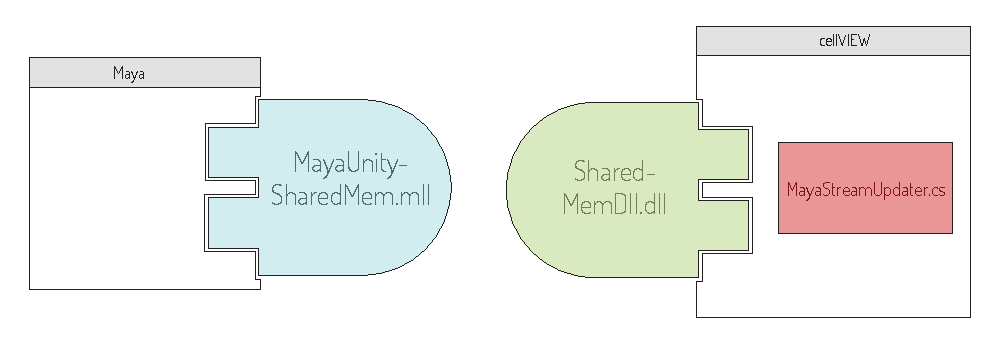
\includegraphics[scale=0.8]{images/system-architecture-overview.pdf}
  \end{center}
  \caption{Overview of system components}
  \label{fig:system-overview}
\end{figure}

% [\textbf{high-level overview of the architecture}]
The architecture of the system consists of three parts - a plugin for Maya, plugin for Unity and a Unity script - as you can see in Figure \ref{fig:system-overview}.
The data flows only in one way - we write into shared memory with Maya plugin and read from shared memory with Unity plugin. This simplifies the situation from the implementation point of view because we don't have to design synchronization scheme.
The plugin for Maya is using Maya API (which will be described later) and is written using in C++ programming language. The function of this plugin is to parse the 3D scene, looking for a molecular objects, and output their positions and rotations (along with info about the instance) into the shared memory.
Unity side of the system consists of two parts - a C++ plugin and a C\# script. The C++ plugin takes care of reading the data from shared memory, while the C\# script, which is a part of cellVIEW, receives this data and uses them to render the final molecular scene. Note that there are two types of interoperability between components: (1) shared memory functionality, which enables two processes to communicate, and (2) interoperability between C++ and C\#, which allows us to pass memory addresses from the plugin to the script on Unity side.

% [\textbf{shared memory} - talk general about shared memory technology]
\section{Shared Memory}
Shared memory is a segment of system memory which can be accessed by multiple programs. It is used as an efficient way to establish communication between separately running processes. Our implementation has been done on Windows, however the concept of shared memory can be found on all operating systems.

% TODO: swaping onto disk, unix, named file mapping in windows
From now on, we will be talking about the implementation that has been done on Windows operating system. There are several way how we can access shared memory here. boost library provides class that provides an abstraction above shared memory functionality. Similarly, Qt framework also has class with comparable function set. We chose to not use any of these. Instead, we directly used Windows API function calls to operate with shared memory. This solution has been chosen because we wanted to use the lowest possible layer because of speed concerns.

\section{C++ and C\# interoperability}

% [\textbf{maya api}]
\section{Maya API}
Maya actually provides two APIs - one in Python[ref] and one in C++[ref]. In addition to that, there is also third way how additional functionality can be implemented - MEL scripting language.

MEL is very similar to other scripting languages like Bash. MEL is not fully mature programming language an therefore is usable only for things like automating tasks that would be otherwise done through the GUI. There is one purpose for which MEL is suitable inside Maya ecosystem - custom GUI creationg. Because of that MEL was not suitable for our job.

Python API is more mature then MEL. Its advantage is that Python, as a interpreted language, can be run without compilation. This means that there doesn't have to be a compilation step and this makes the iteration loop faster. However, we wanted to implemented a functionality that is real-time. This means that we needed every piece of performance we can get. Because of that, the C++ API has been chosen and thus our Maya plugin has been implemented in C++.

There is also another reason why only the C++ route could be taken. We wanted to write into shared memory. The most basic way how to do that is via system API function calls. In our case, we implemented this on Windows platform. Thus the API we used has been WinAPI.

\section{Maya side}
On Maya side, we will talk about the one component that belongs there from our system as can be seen on Figure X.
%Topics - Architecture of the plugin, what parts/classes of API are used, memory layout, what I tried and didn't work.
What we needed to do is basically scan the 3D scene graph and output positions and rotations of each macromolecule object. There are two usecases which needed to be considered. When modeling the scene, the rate of change is not that high. Usually the scene only changes very little (moving or rotating usually just one or few objects). However, we had in mind also a usecase where the animation of the scene would be outputed as well. This means that artist would create a keyframe animation of (nearly) all molecule objects and we would want to transfer the position/rotation data each frame for the animation. Obviously, for each of these use cases there are different ways how to achieve the optimal performance. In the end I settled for (todo: I don't actually know right now)
\section{Unity side}
On the side of cellVIEW (or Unity), we have two components - dll plugin and a C\# script.
Topics - Architecture of the plugin, very generally about plugins (it's just a basic C++ dll plugin), interface between C++ and C\#

\chapter{Demonstration}
In this chapter we present two use cases of how the user can approach illustration with this new proposed system.
Use case one - modified Janet's scene.
Use case two - microtubulus (create a model in maya and then name it properly and we will get it in cellVIEW).

\chapter{Discussion, future work}
The strongest use of the tool as of right now is the live preview of the scene. 

Limitations (of the tool) - what was done just for the use case and should be worked on for final production.
The project has been presented to Drew Berry (I think). Also, it was mention in a talk in Utah, presentation by Peter Mindek.
The method has tremendous potential in its application. The current implementation should be extended for both performance and actual use for artists. For this however, we will need additional input from domain experts. We have been fortunate enough that Drew Berry really liked this work and expressed his desire to develop this project further. It is highly probable that we will be working even more closely with him and that we would continue to improve this system so that he can use it for his movies production.
The challenge will be how to design the system to be easily adaptable by other creators as well.

\appendix %% Start the appendices.
\chapter{Appendix}
Here you can insert the appendices of your thesis.

\newpage
\printbibliography[heading=bibintoc]
\end{document}
